\section*{APPENDIX B - Datasets and code}
\addcontentsline{toc}{section}{APPENDIX B - Datasets and code}
%\addcontentsline{toc}{section}{APPENDIX B - Thesis Planning}
%Time should be allocated to thesis writing and review as well as technical progress.
%A Gantt chart displaying the expected progress over the course of the two semesters
%is shown in \cref{fig:gantt_chart}. Note that a significant portion of time at the beginning was allocated
%to initial research and project scope. Due to the large number of students working on this team,
%a clear project scope was important so that students did not unnecessarily duplicate work.

%\begin{figure}[H]
%    \centering
%    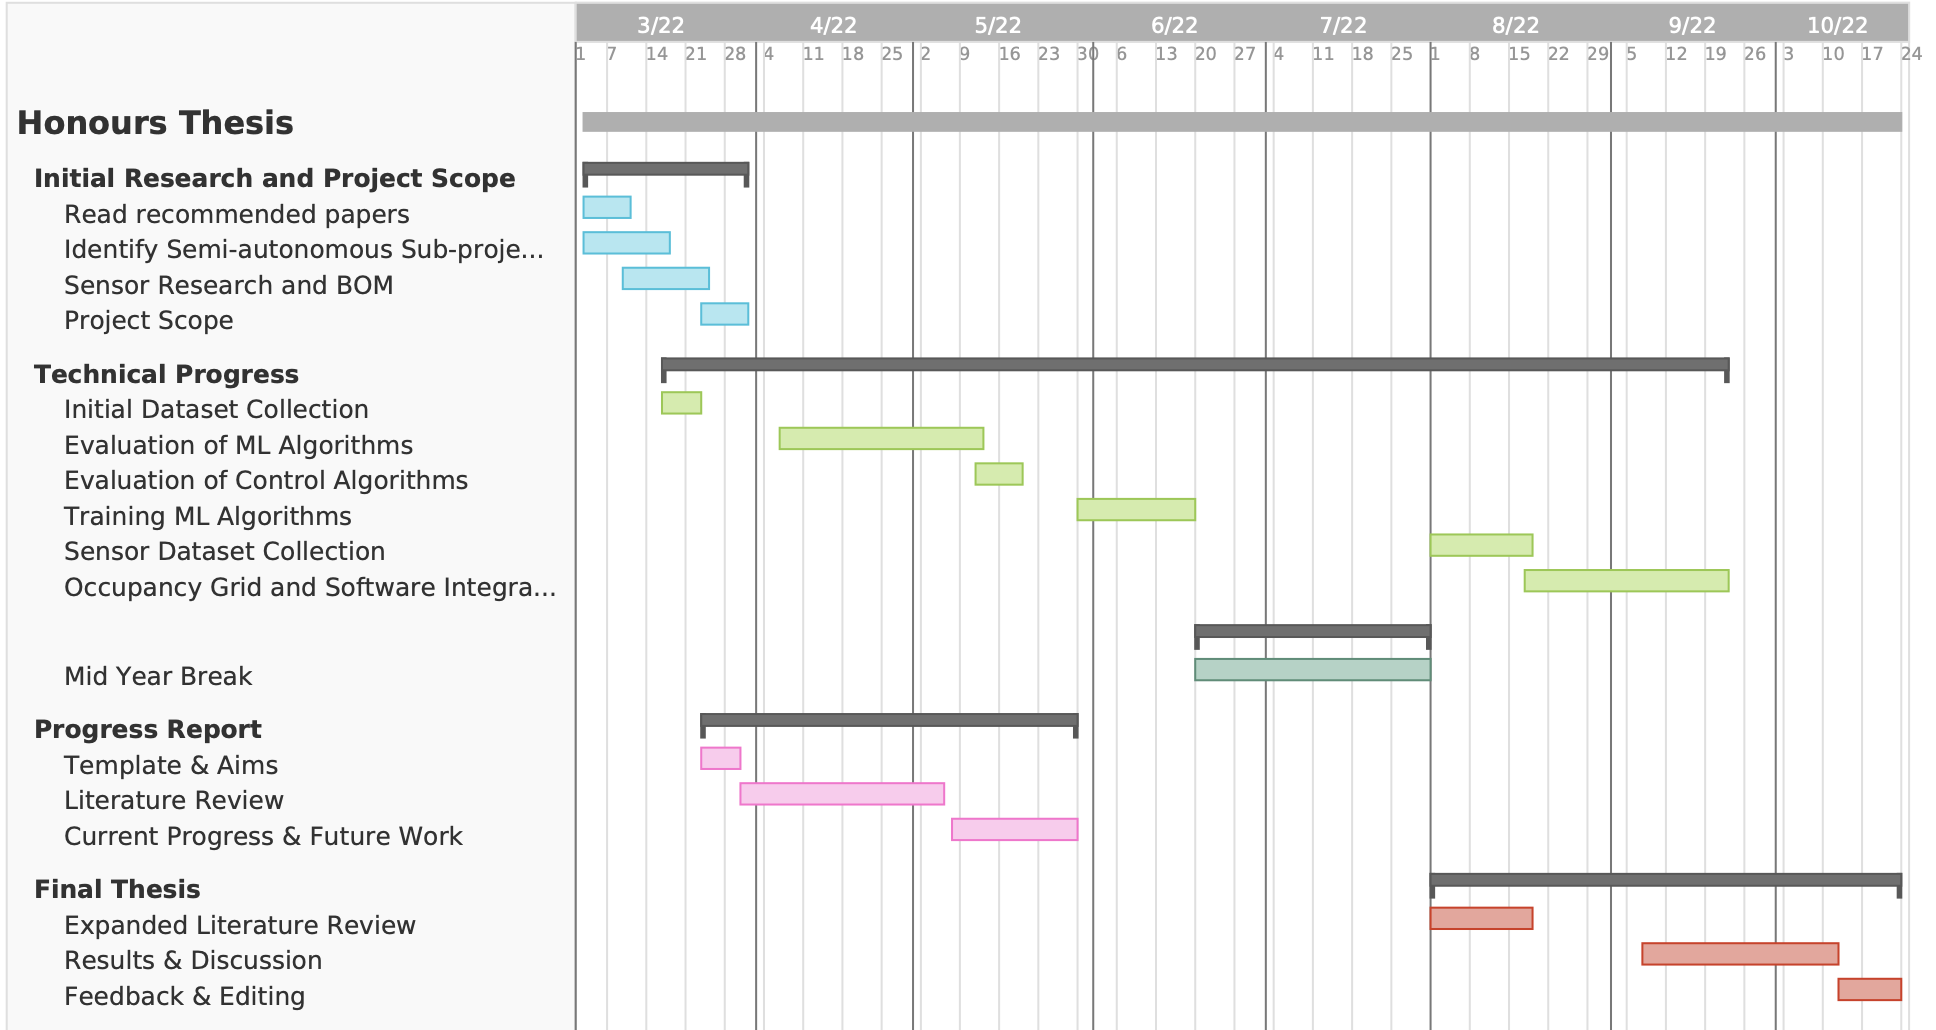
\includegraphics[width=\linewidth]{images/gantt_chart.png}
%    \caption{Gantt chart of thesis progress}
%    \label{fig:gantt_chart}
%\end{figure}
% TODO update Gantt chart

All supplementary material for this thesis has been submitted on a USB thumbdrive.
Some supplementary material has also been uploaded to the 'Curtin X Glide (Smart Wheelchair)' Teams channel so that it can be used by future thesis students
working on this project. Links to each of these files are provided.
\begin{itemize}
    \item The preliminary Curtin University video-only driving dataset is hosted on \href{https://curtin.sharepoint.com/:v:/r/sites/CurtinXGlide/Shared%20Documents/Navigation%20and%20Object%20Detection/GoPro%20Dataset.mp4?csf=1&web=1&e=seLdRb}{\underline{Teams}}.
    \item The ZED Mini RGB-D Curtin University driving dataset is also hosted on \href{https://curtin.sharepoint.com/:f:/r/sites/CurtinXGlide/Shared%20Documents/Navigation%20and%20Object%20Detection/ZED?csf=1&web=1&e=tTau9D}{\underline{Teams}}.
    \item The BDD100K and Cityscapes datasets used to train and evaluate the segmentation model have been uploaded to \href{https://curtin.sharepoint.com/:f:/r/sites/CurtinXGlide/Shared%20Documents/Navigation%20and%20Object%20Detection/External%20Datasets?csf=1&web=1&e=qjWuoP}{\underline{Teams}}.
\end{itemize}

Some material specific to this thesis has also been uploaded to the \href{https://curtin.sharepoint.com/:f:/r/sites/CurtinXGlide/Shared%20Documents/Navigation%20and%20Object%20Detection/Jakob?csf=1&web=1&e=KUuiUt}{\underline{Teams channel}}.
This material includes:
\begin{itemize}
    \item \textbf{datasets/zed/labelled}: Drivable area annotations for a portion of the Curtin RGB-D driving dataset. Refer to appendix D for further information.
    \item \textbf{datasets/zed/video}: The Curtin RGB-D driving dataset converted into the avi video format, for use with devices that may not have the ZED SDK installed.
    \item \textbf{models}: Model weights for trained ML models, saved at each training epoch.
    \item \textbf{results}: Video results for segmentation, obstacle detection, and assistive control algorithms (tested on the Curtin RGB-D driving dataset).
\end{itemize}

All code used in this thesis can be found on \href{https://github.com/JakobWyatt/smart-wheelchair}{\underline{Github}}.
This repository contains:
\begin{itemize}
    \item \textbf{code}: Python and MATLAB code used to implement various algorithms.
    \item \textbf{colab}: Colab notebooks used to train the segmentation model.
    \item \textbf{environments}: Conda environments used to manage dependencies.
    \item \textbf{models}: 3D models for the ZED mount (Inventor, Fusion, STL).
    \item \textbf{repositories}: Git submodules and sample code.
\end{itemize}
This repository also contains the latex source code used to format this document.
